
%\documentstyle[boxedminipage,alltt,psfig,epsf,pvs]{llncs}

\documentclass{llncs}

\usepackage{chngcntr}
\usepackage{graphicx}
\usepackage{boxedminipage,alltt,psfig,epsf,pvs}
% Derived from John Rushby's prelude.tex, modified for NFSS2
%
% define variants of the \LaTeX macro that avoid using \sc
% for use in headings
%

% Define fonts that work in math or text mode
\def\dwimrm#1{\ifmmode\mathrm{#1}\else\textrm{#1}\fi}
\def\dwimsf#1{\ifmmode\mathsf{#1}\else\textsf{#1}\fi}
\def\dwimtt#1{\ifmmode\mathtt{#1}\else\texttt{#1}\fi}
\def\dwimbf#1{\ifmmode\mathbf{#1}\else\textbf{#1}\fi}
\def\dwimit#1{\ifmmode\mathit{#1}\else\textit{#1}\fi}
\def\dwimnormal#1{\ifmmode\mathnormal{#1}\else\textnormal{#1}\fi}

\def\BigLaTeX{{\rm L\kern-.36em\raise.3ex\hbox{\smaller\smaller A}\kern-.15em
    T\kern-.1667em\lower.7ex\hbox{E}\kern-.125emX}}
\def\BoldLaTeX{{\bf L\kern-.36em\raise.3ex\hbox{\smaller\smaller\bf A}\kern-.15em
    T\kern-.1667em\lower.7ex\hbox{E}\kern-.125emX}}
%\def\labelitemi{$\bullet$}
\def\labelitemii{$\circ$}
\def\labelitemiii{$\star$}
\def\labelitemiv{$\diamond$}
\newcommand{\tcc}{{\smaller\smaller TCC}}
\newcommand{\tccs}{\tcc s}
\newcommand{\emacs}{{E{\smaller\smaller MACS}}}
\newcommand{\Emacs}{\emacs}
\newcommand{\ehdm}{{E{\smaller\smaller HDM}}}
\newcommand{\Ehdm}{\ehdm}
\newcommand{\tm}{$^{\mbox{\tiny TM}}$}
\newcommand{\hozline}{{\noindent\rule{\textwidth}{0.4mm}}}

\newcommand{\allclear}%
  {\mbox{\boldmath$\stackrel{\raisebox{-.2ex}[0pt][0pt]%
              {$\textstyle\oslash$}}{\displaystyle\bot}$}}

\newenvironment{private}{}{}

\newenvironment{smalltt}{\begin{alltt}\small}{\end{alltt}}

\newlength{\hsbw}

\newenvironment{session}%
  {\begin{flushleft}
   \setlength{\hsbw}{\linewidth}
   \addtolength{\hsbw}{-\arrayrulewidth}
   \addtolength{\hsbw}{-\tabcolsep}
   \begin{tabular}{@{}|c@{}|@{}}\hline 
   \begin{minipage}[b]{\hsbw}
   \begingroup\small\mbox{ }\\[-1.8\baselineskip]\begin{alltt}}
  {\end{alltt}\endgroup\end{minipage}\\ \hline 
   \end{tabular}
   \end{flushleft}}

\newenvironment{smallsession}%
  {\begin{flushleft}
   \setlength{\hsbw}{\linewidth}
   \addtolength{\hsbw}{-\arrayrulewidth}
   \addtolength{\hsbw}{-\tabcolsep}
   \begin{tabular}{@{}|c@{}|@{}}\hline 
   \begin{minipage}[b]{\hsbw}
   \begingroup\footnotesize\mbox{ }\\[-1.8\baselineskip]\begin{alltt}}%
  {\end{alltt}\endgroup\end{minipage}\\ \hline 
   \end{tabular}
   \end{flushleft}}

\newenvironment{spec}%
  {\begin{flushleft}
   \setlength{\hsbw}{\textwidth}
   \addtolength{\hsbw}{-\arrayrulewidth}
   \addtolength{\hsbw}{-\tabcolsep}
   \begin{tabular}{@{}|c@{}|@{}}\hline 
   \begin{minipage}[b]{\hsbw}
   \begingroup\small\mbox{ }\\[-0.2\baselineskip]}%
  {\endgroup\end{minipage}\\ \hline 
   \end{tabular}
   \end{flushleft}}

\newcommand{\memo}[1]%
  {\mbox{}\par\vspace{0.25in}%
   \setlength{\hsbw}{\linewidth}\addtolength{\hsbw}{-1.5ex}%
   \noindent\fbox{\parbox{\hsbw}{{\bf Memo: }#1}}\vspace{0.25in}}

\newcommand{\nb}[1]%
  {\mbox{}\par\vspace{0.25in}%
   \setlength{\hsbw}{\linewidth}\addtolength{\hsbw}{-1.5ex}%
   \noindent\fbox{\parbox{\hsbw}{{\bf Note: }#1}}\vspace{0.25in}}

\newcommand{\comment}[1]{}
\newcommand{\exfootnote}[1]{}
%\newcommand{\ifelse}[2]{#1}
\sloppy
\clubpenalty=100000
\widowpenalty=100000
%\displaywidowpenalty=100000
\setcounter{secnumdepth}{3} 
\setcounter{tocdepth}{3}
\setcounter{topnumber}{9}
\setcounter{bottomnumber}{9}
\setcounter{totalnumber}{9}
\renewcommand{\topfraction}{.99}
\renewcommand{\bottomfraction}{.99}
\renewcommand{\floatpagefraction}{.01}
\renewcommand{\textfraction}{.2}
\font\largett=cmtt10 scaled\magstep1
\font\Largett=cmtt10 scaled\magstep2
\font\hugett=cmtt10 scaled\magstep3

%\renewcommand{\memo}[1]{\mbox{}\par\vspace{0.25in}\noindent\fbox{\parbox{.95\linewidth}{{\bf Memo: }#1}}\vspace{0.25in}}

\newcommand{\eg}{{\em e.g.\/},}
\newcommand{\ie}{{\em i.e.\/},}

\newcommand{\pvs}{PVS}

\newcommand{\ch}{\choice}
\newcommand{\rsv}[1]{{\rm\tt #1}}

\newcommand{\lpvstheory}[3]{\figurehead{\hozline\smaller\smaller\begin{alltt}}%
			   \figuretail{\end{alltt}\vspace{-0in}\hozline}%
			   \figurelabel{#3}\figurecap{#2}%
			   \begin{longfigure}\input{#1}\end{longfigure}}

\newcommand{\pvstheory}[3]
  {\begin{figure}[htb]\begin{boxedminipage}{\textwidth}%
   {\smaller\smaller\begin{alltt} \input{#1}\end{alltt}}\end{boxedminipage}%
   \caption{#2}\label{#3}\end{figure}}

\newcommand{\bpvstheory}[3]
  {\begin{figure}[b]\begin{boxedminipage}{\textwidth}%
   {\smaller\smaller\begin{alltt} \input{#1}\end{alltt}}\end{boxedminipage}%
   \caption{#2}\label{#3}\end{figure}}

\newcommand{\spvstheory}[1]
  {\vspace{0.1in}\par\noindent\begin{boxedminipage}{\textwidth}%
   {\smaller\smaller\begin{alltt} \input{#1}\end{alltt}}\end{boxedminipage}\vspace{0.1in}%
   }
%\newenvironment{spvstext}%
%  {\vspace{0.1in}\par\noindent\begin{boxedminipage}{\textwidth}%
%   \smaller\smaller\begin{alltt}}%
%  {\end{alltt}\end{boxedminipage}\vspace{0.1in}%
%   }


%  {\begin{boxedminipage}{\textwidth}{\smaller\smaller\begin{alltt}#1\end{alltt}}\end{boxedminipage}}
%\newenvironment{spvstheory}{\par\noindent\begin{boxedminipage}{\textwidth}\smaller\smaller\begin{alltt}}{\end{alltt}\end{boxedminipage}}

\newenvironment{pvsex}%
  {\setlength{\topsep}{0in}\smaller\begin{alltt}}%
  {\end{alltt}}

\newcommand{\pvsbnf}[2]
  {\begin{figure}[htb]\begin{boxedminipage}{\textwidth}%
   \input{#1}\end{boxedminipage}\caption{#2}\label{#1}\end{figure}}

\newcommand{\spvsbnf}[1]
  {\begin{boxedminipage}{\textwidth}\input{#1}\end{boxedminipage}}

\newcommand{\pidx}[1]{{\rm #1}}	% primary index entry
\newcommand{\sidx}[1]{{\rm #1}} % secondary index entry
\newcommand{\cmdindex}[1]{\index{#1@\cmd{#1}}}
\newcommand{\icmd}[1]{\cmd{#1}\cmdindex{#1}}
\newcommand{\iecmd}[1]{\ecmd{#1}\cmdindex{#1}}

\newenvironment{pvscmds}%
  {\par\noindent\smaller%
   \begin{tabular*}{\textwidth}{|l@{\extracolsep{\fill}}ll|}\hline%
     {\it Command} & {\it Aliases} & {\it Function}\\ \hline}%
  {\hline\end{tabular*}\vspace{0.1in}}

\newcommand{\cmd}[1]{{\tt #1}}
\newcommand{\ecmd}[1]{{\tt M-x #1}}

\newcommand{\latex}{\LaTeX}                  %  LaTeX
\newcommand{\sun}{{S{\smaller\smaller UN}}}                 %  Sun
\newcommand{\sparc}{{S{\smaller\smaller PARC}}}             %  Sparc
\newcommand{\sunos}{{S{\smaller\smaller UN}OS}}             %  SunOS
\newcommand{\solaris}{{\em Solaris\/}}        %  Solaris
\newcommand{\sunview}{{S{\smaller\smaller UN}V{\smaller\smaller IEW}}} %SunView
\newcommand{\unix}{{U{\smaller\smaller NIX}}}               %  Unix
\newcommand{\lisp} {{\sc Lisp}}              %  Lisp
\newcommand{\gnu}{{\sc Gnu Emacs}}           %  Gnu Emacs
\newcommand{\gnuemacs}{{\sc Gnu Emacs}}      %  Gnu Emacs
\newcommand{\emacsl}{{\sc Emacs-Lisp}}       %  Emacs Lisp
\newcommand{\shell}{{\sc Csh}}               %  C-shell

\newcommand{\update}[3]{#1\{#2\leftarrow #3\}}
\newcommand{\interp}[3]{\cal{M}\dlb {\tt #1 : #2 }\drb #3}
\newcommand{\myforall}[2]{(\forall{#1 .}\ #2)}
\newcommand{\myexists}[2]{(\exists{#1 .}\ #2)}
\newcommand{\mth}[1]{$ #1 $}
\newcommand{\labst}[2]{(\lambda{#1}.\ #2)}
\newcommand{\app}[2]{(#1\ #2)}
%\newcommand{\problem}[1]{{\bf Exercise: } {\em #1}}
\newcommand{\rectype}[1]{[\# 1 \#]}
\newcommand{\recttype}[1]{{\tt [\# 1 \#]}}
\newcommand{\dlb}{\lbrack\!\lbrack}
\newcommand{\drb}{\rbrack\!\rbrack}
\newcommand{\cross}{\times}
\newcommand{\key}[1]{{\tt #1}}
\newcommand{\keyword}[1]{{\smaller\texttt{#1}}}

\newenvironment{keybindings}%
  {\begin{center}\begin{tabular}{|l|l|}\hline Key & Function\\ \hline}%
  {\hline\end{tabular}\end{center}}
\def\rmif{\mbox{\bf if\ }}
\def\rmiff{\mbox{\bf \ iff \ }}
\def\rmthen{\mbox{\bf \ then }}
\def\rmelse{\mbox{\bf \ else }}
\def\rmend{\mbox{\bf end}}
\def\rmendif{\mbox{\bf \ endif}}
\def\rmotherwise{\mbox{\bf otherwise}}
\def\rmwith{\mbox{\bf \ with\ }}


\newcommand{\refines}{\ll}
\newcommand{\andthen}{\wedge}
\newcommand{\implies}{\Longrightarrow}
\newcommand{\chap}[2]{\clearpage\mbox{}\clearpage\chapter{#1}\label{#2}}
\newcommand{\Murphi}{Mur$\phi$}
\newcommand{\MuC}{$\mu$-calculus}
\newcommand{\PVS}{PVS}
\newcommand{\name}[1]{{\rm #1}}
\newcommand{\todo}[1]{\ldots {\Large #1}}
%%%\newtheorem{definition}{Definition}[section]
%%%\newtheorem{theorem}{Theorem}[section]
%%%\newtheorem{remark}{Remark}[section]
%\newenvironment{proof}
%  {{\bf Proof}}
%  {\qed}
%\def\bull{\vrule height.9ex width.8ex depth-.1ex}
%\newcommand{\qed}{{\hbox{}\hfill\bull\normalsize\medbreak}}


%%% Local Variables: 
%%% mode: latex
%%% TeX-master: t
%%% End: 


\renewenvironment{smallsession}
 {\begin{flushleft}%
  \setlength{\hsbw}{\linewidth}%
  \begin{boxedminipage}[b]{\hsbw}%
  \begingroup\small%
  \begin{alltt}}%
 {\end{alltt}\endgroup\end{boxedminipage}\end{flushleft}}

\pagestyle{plain}

\begin{document}

\title{A Refinement Proof for a Garbage Collector}

\author{ 
Klaus Havelund\inst{2}\thanks{Part of the research performed by 
his author was carried out at Jet Propulsion Laboratory, California 
Institute of Technology, under a contract with the National Aeronautics 
and Space Administration.}
\and
Natarajan Sjankar\inst{1}
}

\institute{
Jet Propulsion Laboratory, \\
California Institute of Technology, Pasadena, USA 
\and
Computer Science Laboratory,\\
SRI International, Menlo Park, USA
}

% Klaus's original support:
% -------------------------
% Supported by a European Community HCM grant 
% while working at LITP, Paris 6, France; and by the Danish BRICS project 
% while working at Aalborg University. 

% Shankar's original support:
% ---------------------------
% Supported by NSF Grant CCR-930044
% and by ARPA through NASA Ames Research Center under Contract
% NASA-NAG-2-891 (ARPA Order A721).


\maketitle

%\begin{keywords}
%Garbage Collector;
%Concurrency;
%Program Verification;
%State Transition Systems;
%Refinement;
%Theorem Proving; 
%PVS. 
%\end{keywords}

% Master File: main.tex

\begin{abstract}
  
  We describe how the PVS verification system  has been used to verify
  a  safety  property of a widely studied garbage collection  algorithm.
  The safety property  asserts  that    ``nothing  but garbage  is    ever
  collected.''  The garbage  collection algorithm and  its composition
  with  the user program can be regarded  as a concurrent  system with two
  processes working on  a shared memory.   Such concurrent systems can be
  encoded in  PVS as state transition systems using a
  model similar to TLA~\cite{TLA:TOPLAS94}.  The  safety  criterion is
  formulated  as a 
  refinement and proved  using  refinement  mappings.    
  Russinoff~\cite{Rus:GC}  originally verified the algorithm   in  the Boyer-Moore
  prover, but his proof was not  based on refinement and 
  safety property  cannot be appreciated  without a  glass box view of
  the   workings of the algorithm.    Using
  refinement, however,  the safety criterion makes sense independent of
  the garbage collection algorithm.   As a by-product, we encode  a
  a version of the theory of refinement mappings in PVS. The paper reflects
  substantial work that was done over two decades ago, but which is still relevant.
  
\end{abstract}

%%% Local Variables: 
%%% mode: latex
%%% TeX-master: t
%%% End: 




         
\section{Introduction}

Russinoff~\cite{Rus:GC} used   the Boyer-Moore theorem prover  to
verify  a  safety  property   of   a {\em  mark--and--sweep}   garbage
collection  algorithm originally suggested  by Ben-Ari \cite{Ben:GC}. 
The garbage collector and   its composition with   a user  program  is
regarded as a concurrent system with both processes working on
a common shared memory.  The  collector uses a colouring  (marking) technique
to iteratively colour all accessible nodes {\em black} while 
leaving garbage nodes {\em white}.  When the colouring has
stabilized, all the white nodes can be collected and placed in the
free list.

An initial  version of the algorithm  was  first proposed by Dijkstra,
Lamport, Martin, Scholten, and Steffens~\cite{DLMSS:GC} as an exercise
in  organizing and verifying the cooperation  of concurrent processes. 
Their solution   involved   three  colours.   Ben-Ari    improved this
algorithm so  as  to use    only  two colours  while  simplifying  the
resulting proof.  All of these  proofs were  informal {\em pencil  and
  paper\/} exercises.  As   pointed  out by   Russinoff~\cite{Rus:GC},
these informal proofs  ran into difficulties  of one sort or  another. 
Dijkstra, et al~\cite{DLMSS:GC}    explained   (as an  example  of   a
``logical trap'') how they originally proposed a minor modification to
the  algorithm.   This claim turned   out  to   be  wrong, and  was
discovered by the authors just  before the proof reached publication.  
Ben-Ari  later  proposed the same  modification   to his algorithm and
argued for   its    correctness   without  discovering its       flaw. 
Counterexamples    were  later  given    by  Pixley~\cite{Pix:GC}  and
van~de~Snepscheut~\cite{Van:GC}.   Furthermore,  although    Ben-Ari's
algorithm 
%(which is the one we verify in PVS) 
is correct, his proof of
the safety property was found to be flawed.  This flaw was essentially
reproduced by Pixley \cite{Pix:GC} where it  again survived the  review
process, and was only discovered  ten years later by Russinoff  during
the course of his mechanical verification~\cite{Rus:GC}.  Ben-Ari also
gave a flawed  proof of a liveness  property ({\em every garbage  node
  will eventually be collected}) that was later observed and corrected
by van~de~Snepscheut~\cite{Van:GC}.

Russinoff's correctness property is formulated as a  state predicate $P$, which
is then proven to be an invariant, i.e., true in all reachable  states.
In gross  terms, 
this invariant predicate is formulated as  follows.  The garbage collector
can at 
any time be in one of 9 different locations.  In one of the locations,
here  called {\sc  Append},  the {\em append} operation  representing
garbage collection is applied to a certain  memory node $X$, but only
when this node is white. The safety  predicate  $P$  is  then formulated  as:
%
{\em ``if the control of the garbage collector is at 
location {\sc Append} and
$X$ is white then $X$ is garbage''}.
%
%\begin{center}
%  {\em If the control of the garbage collector is at\\ 
%  location {\sc Append} and
%  $X$ is white then $X$ is garbage} 
%\end{center}
%
%\noindent
However, this formulation of   the  safety property does not really  tell us
whether the  program is correct.  We 
have to additionally ensure that  the {\em append} operation is
only invoked in location {\sc Append}, and only on white nodes.  Hence,
the safety property of the garbage collector follows from both the
invariance of $P$ and an operational understanding of the
garbage collection algorithm.  

This  observation motivated  us  to  carry  out a   proof  in the PVS\footnote{PVS stands for Prototype Verification System.} theorem prover
\cite{pvs-url} using   a  refinement approach,  presented in this paper,
where   the safety property  itself  is formulated  as an  abstract algorithm, and
the proof  is  based  on refinement  mappings  as suggested  by
Lamport~\cite{TLA:TOPLAS94}.  This  approach   has the advantage  that  the
safety property can  be formulated more abstractly without considering
the internal structure of the final implementation.  Here a {\em black
  box} view   of the  algorithm is   sufficient.  This yields a
further contribution in terms of the 
formalization of refinement mappings in PVS.
In  order   better to make  a
comparison, we also carried out a proof in PVS using the same
technique   as  in~\cite{Rus:GC}.  This    work   was documented  in
\cite{havelund-pvs-gc-99}.
%
In~\cite{HS:BRP}  we verified  a  distributed communication  protocol
using similar techniques for representing  state transition systems. 
%The work  presented here can therefore be   seen as part 
%of a series of  PVS verifications of parallel/distributed 
%algorithms, carried out to establish a framework for such 
%verifications, while
%identifying the main difficulties  in carrying  out such
%proofs. 
Our  key conclusion  is  that  techniques for
strengthening invariants are  of major importance also in refinement
proofs, and that refinement does not remove this burden.  
%
The proof presented here was carried out over two decades ago, but
was only published as a (substantial) technical report \cite{havelund-shankar-gc-report-97}. 
Since we still consider the work relevant, and even
cited, we decided to finally publish this work.

The paper is organized as follows.
Section \ref{sec:related-work} 
outlines additional related work.
In  Section~\ref{transition-systems},  a    formalization of state
transition  systems and  refinement mappings  is  provided in  an informal
mathematical style that  is  later formalized  in  PVS.  The garbage
collection algorithm is described in
Section~\ref{informal-specification}\@.
Sections~\ref{goto-specification} and~\ref{refinement-steps} present
the successive refinements of the initial algorithm in three stages.
This presentation is based on   an informal notation for  transition systems.
Section~\ref{observations} lists some observations on the entire
verification exercise. 
Appendices \ref{pvs-specifications} and \ref{pvs-proof} formalize
the concepts  introduced   in   Sections~\ref{transition-systems},
\ref{goto-specification} and~\ref{refinement-steps} in PVS.   

%%% Local Variables: 
%%% mode: latex
%%% TeX-master: t
%%% End: 




\section{Transition Systems and Refinement Mappings}
\label{transition-systems}

In this section,  we establish the  formal theory for using an abstract
non-deterministic program as   a safety specification so  that any
behaviour is safe as long as it is generated by the program.  An implementation
is then defined as  a refinement of  this program.  The basic concepts
are those of {\em transition systems}, {\em traces}, {\em invariants},
{\em  observed  transition   systems},   {\em refinements},   and {\em
  refinement mappings}.  The  theory presented is a minor modification
of the theory developed by Abadi and Lamport~\cite{AL:Mappings}, 
with some modest differences.     We first introduce   the basic concept of  a
transition system.  Specifications as  well as their refinements
are written as transition systems.

\begin{definition}[Transition System]
A transition system is a triple $(\Sigma,I,N)$, where

\begin{itemize}

  \item $\Sigma$ is a {\em state} space

  \item $I \subseteq \Sigma$ is the set of {\em initial} states.

  \item $N \subseteq \Sigma \times \Sigma$ is the {\em next-state} relation.
        Elements of $N$ are denoted by pairs of the form $(s,t)$, meaning that
        there is a transition from the state $s$ to the state $t$.

\end{itemize}
\end{definition}

\noindent
An {\em execution trace\/}  is an infinite sequence of
states,  where  the first state  satisfies  the initiality predicate and
every pair  of adjacent states is  related  by the  next-state
relation.  A 
sequence $\sigma$  is just an infinite enumeration  of states $\langle s_0,
s_1,  s_2, \ldots \rangle$.     We  let $\sigma_i$ denote  the  $i$'th
element $s_i$  of the  sequence.    The traces of   a transition
system can be defined as follows.

\begin{definition}[Traces]
\label{def-traces}
  The traces of a transition system are defined as follows:

\[
\Theta(\Sigma,I,N) = \{ \sigma \in \Sigma^{\omega} \mid 
                          \sigma_0 \in I \wedge
                          \forall i \ge 0 \cdot N(\sigma_i,\sigma_{i+1}) \}
\] 
\end{definition}

\noindent
We shall need the notion of a  transition system invariant, which is
a state predicate true  in all states reachable  from an initial state
by following the transition relation.

\begin{definition}[Invariant]
\label{def-invariants}
Given a transition system $S = (\Sigma,I,N)$, then a predicate 
$P : \Sigma \rightarrow {\cal B}$ is an $S$ invariant iff.

\[
\forall \sigma \in \Theta(S) \cdot 
\forall i \ge 0 \cdot P(\sigma_i)
\]

\end{definition}

\noindent
Since we want to compare transition systems, and decide whether one transition
system refines another, we need a notion of {\em observability}.
For that purpose, we extend transition systems with an {\em observation 
function}, which when applied to a state returns an observation in some domain.

\begin{definition}[Observed Transition System]
\label{def-observed-transition-system}  
An        observed  transition      system      is  a     five-tuple
$(\Sigma,\Sigma_o,I,N,\pi)$ where

\begin{itemize}

  \item $(\Sigma,I,N)$ is a transition system

  \item $\Sigma_o$ is a state space, the observed one

  \item $\pi : \Sigma \rightarrow \Sigma_o$ is an {\em observation function}
        that extracts the observed part of a state.

\end{itemize}
\end{definition}

\noindent
Typically (at least in our case) a state  $s \in \Sigma$ consists
of an   observable  part $s_{obs} \in \Sigma_o$  and  an  internal part
$s_{int}$, hence $s = (s_{obs},s_{int})$ and $\pi$ is just the
projection function: $\pi(s_{obs},s_{int}) = s_{obs}$.
We adopt the convention that a projection  function $\pi$ applied to a
trace $\langle s_1,  s_2, \ldots \rangle$ results in  the
projected trace $\langle \pi(s_1), \pi(s_2), \ldots \rangle$.

The central concept in all this is  the notion of refinement: that one
observed transition system  $S_2$ refines  another observed transition
system $S_1$.  By  this we intuitively mean  that every observation we
can make on  $S_2$,  we can  also make on   $S_1$.  Hence,  if  $S_1$
behaves safely so will $S_2$ since every projected  trace of $S_2$ is  a
projected trace  of $S_1$.  
This is formulated in the following definition.

\begin{definition}[Refinement]
\label{def-refinement}
An observed transition system\\ 
  $S_2$ $=$ $(\Sigma_2,\Sigma_o,I_2,N_2,\pi_2)$ 
{\em refines} an observed transition system   
  $S_1$ $=$ $(\Sigma_1,\Sigma_o,I_1,N_1,\pi_1)$ 
iff (note that they have the same observed state space $\Sigma_o$):

\[
  \forall \sigma_2 \in \Theta(S_2) \cdot 
    \exists \sigma_1 \in \Theta(S_1) \cdot
      \pi_1(\sigma_1) = \pi_2(\sigma_2)
\]
\end{definition}

\noindent
We have thus established  what it means for one  observed transition
system to refine another, but we still need  a  practical way of
showing refinement.  Note  that 
refinement is defined in terms of traces which are infinite objects
so that reasoning about them directly is impractical.  We need a way  of
reasoning  about states and pairs of states. A {\em refinement mapping} is
a suitable tool for this purpose.  A 
refinement  mapping from  a  lower  level  transition system $S_2$ to   a
higher-level  one $S_1$ is    a mapping from the state space  $\Sigma_2$ to
the  state space $\Sigma_1$, that when applied statewise, 
maps traces of $S_2$ to traces of $S_1$.  This is formally stated as
follows.

\begin{definition}[Refinement Mapping]
\label{def-refinement-mapping}
A {\em refinement mapping} from an observed transition system
  $S_2 = (\Sigma_2,\Sigma_o,I_2,N_2,\pi_2)$
to an observed transition system
  $S_1 = (\Sigma_1,\Sigma_o,I_1,N_1,\pi_1)$
is a mapping $f : \Sigma_2 \rightarrow \Sigma_1$ such that there exists an
$S_2$ invariant $P$,  where:

\begin{enumerate}

 \item $\forall s \in \Sigma_2 \cdot \pi_1(f(s)) = \pi_2(s)$

 \item $\forall s \in \Sigma_2 \cdot I_2(s) \Rightarrow I_1(f(s))$

 \item $\forall s,t \in \Sigma_2 \cdot 
          P(s) \wedge P(t) \wedge N_2(s,t) \Rightarrow N_1(f(s),f(t))$ 
       
\end{enumerate}
\end{definition}

\noindent
We   can now    state   the  main   theorem   (which  is   stated   in
\cite{AL:Mappings}, and which we have proved in  PVS for our slightly
modified version):

\begin{theorem}[Existence of Refinement Mappings]
\label{theorem-refinement}
If there exists a refinement mapping from an observed transition system $S_2$
to an observed transition system $S_1$, then $S_2$ refines $S_1$. 

\end{theorem}

We shall show how we demonstrate the  existence of refinement mappings
in PVS,  by providing a {\em witness},  that is: defining a particular
one. Defining the refinement mapping  turns out typically to be  easy,
whereas showing that it is indeed a refinement mapping (the properties
in Definition~\ref{def-refinement-mapping}) is  where the  major  effort
goes.  Especially finding and proving the invariant $P$ is the bulk of
the proof.

We   differ from Abadi  and Lamport~\cite{AL:Mappings} in two
ways.  First, we allow general  observation functions, and not
just projection functions that are the identity map on a subset of   the
state space.   Second, in Definition~\ref{def-refinement-mapping} of
refinement mappings,  we  assume that states  $s$  and $t$  satisfy an
implementation     invariant  $P$,   which    is   not   the  case
in~\cite{AL:Mappings}\@.   We have thus weakened the premises of
the refinement rule.  Whereas the introduction of observation functions
is just a nice (but not   strictly   necessary) generalization,
the use of invariants is of real importance for practical proofs.

%%% Local Variables: 
%%% mode: latex
%%% TeX-master: t
%%% End: 








         
\section{The Algorithm}
\label{informal-specification}

In  this  section   we  informally  describe the   garbage  collection
algorithm.   As illustrated  in    Figure~\ref{gc-figure}, the  system
consists of two processes, the  {\em mutator} and the {\em collector},
working on a shared {\em memory}.

\begin{figure}[htb]
\center
%\makebox[\textwidth]{\epsfbox{gc-fig.ps}}
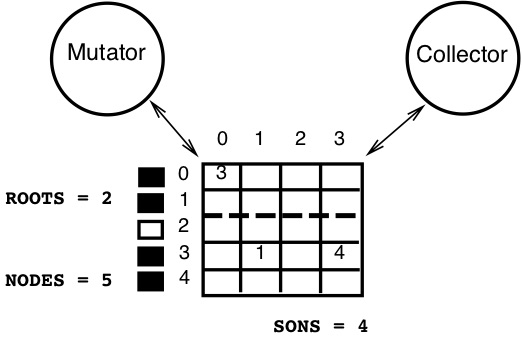
\includegraphics[width=2.5in]{gc-fig.jpeg}
\caption{The mutator, collector and shared memory}
\label{gc-figure}
\end{figure}

\subsection{The Memory}

The memory is a fixed size array of  {\em nodes}.  In
Figure~\ref{gc-figure} there 
are 5 nodes (rows) numbered 0--4.  Associated with  each node is an
array of uniform  length of {\em cells}.     Figure~\ref{gc-figure} shows
4 cells numbered 0 -- 3 per node.  A cell is  identified by a pair
of  integers ($n$,$i$) where  $n$ is  a node number  and where  $i$ is
called   the {\em index}.   Each  cell  contains a pointer   to a node,
called the {\em son}.  In the case   of a LISP  implementation, there  are, for
example, two  cells per node.  In   Figure~\ref{gc-figure}, we  assume
that all empty 
cells contain  the  {\em NIL} value 0,   and hence point to   node 0.  In
addition, node 0 points to node 3 (because  cell (0,0) does so), which
in turn points to nodes 1 and  4.  Hence the memory  can be thought of
as a two-dimensional  array, the  size of  which is  determined by the
positive integer constants  {\tt NODES} and {\tt  SONS}\@.   Each node
has an  associated  {\em colour},  black or white,  that  is used by the
collector in identifying garbage nodes.

A pre-determined number of   nodes, defined  by the positive   integer
constant {\tt  ROOTS}, are designated  as the  {\em roots},  and these are
kept in the initial  part  of the array (they   may be thought of   as
static program variables).   In  Figure~\ref{gc-figure}, there  are two
such  roots shown separated from the rest with a dotted line. A node is {\em
accessible} 
if it can be reached from a root by  following pointers, and a node is
{\em garbage} if it is not accessible. Nodes 0, 1, 3, and 
4  in Figure~\ref{gc-figure} are therefore accessible, and node 2 is
garbage. 

\noindent There  are  only three operations by which
the memory structure can be modified:

\begin{itemize}
  \item Redirect a pointer towards an accessible node.
  \item Change the colour of a node.
  \item Append a garbage node to the free list.
\end{itemize}

\noindent In the initial state, all pointers are assumed to  be 0, 
and nothing is assumed about the colours.


\subsection{The Mutator}

The mutator  corresponds to  the user  program  and performs the  main
computation.  From an abstract point of  view, it continuously changes
pointers  in the memory; the   changes being arbitrary except for  the
fact that  a cell can  only be set to point  to an  already accessible
node. In  changing a  pointer  the ``previously pointed-to'' node  may
become garbage,  if it  is  not accessible   from  the roots  in  some
alternative way.  In  Figure~\ref{gc-figure}, any cell can hence be
modified by the 
mutator to point to a node other than  2.  Only
accessible  cells can be modified, but as shown below,  the algorithm can
in fact be proved safe  without this restriction.  The algorithm is as
follows: 
\begin{enumerate}

\item Select a node $n$, an index $i$, and an accessible node $k$,
      and assign $k$ to cell ($n$,$i$). 
      
\item Colour node $k$ black. Return to step 1.

\end{enumerate}

\noindent Each of the two steps is regarded as an atomic instruction.


\subsection{The Collector}

The collector collects  garbage nodes and  puts
them into  a {\em free list}, from  which the  mutator may then remove
them as they are needed during dynamic storage allocation.  Associated
with each node is a {\em colour} field, that is used  by the collector
during  its  identification of garbage  nodes.  Basically,  it colours
accessible nodes {\em  black}, and at  a certain point it collects all
{\em white} nodes, which are then garbage, and puts them into the free
list. Figure~\ref{gc-figure} illustrates the situation at such a  point:
only node  2 is white since  it is the only garbage node.  The collector
algorithm is as follows:
%
\label{the-collector-informal}
\begin{enumerate}

\item Colour each root black.

\item Examine each pointer in succession. If the source is black and the
      target is white, colour the target black.

\item Count the black nodes. If the result exceeds the previous count (or
      if there was no previous count), return to step 2.

\item Examine each node in succession. If a node is white, append it to
      the free list; if it is black, colour it white. Then return to step 1.

\end{enumerate}

\noindent
Steps 1--3 constitute the {\em marking}  phase where 
all accessible   nodes are blackened.  Each of these steps involves an
iteration involving a smaller step that is executed atomically.  
For example,  step~3
consists   of several atomic instructions,  each  counting (or not) a
single node.


%%% Local Variables: 
%%% mode: latex
%%% TeX-master: t
%%% End: 


\section{The Specification}
\label{goto-specification}

We now present  the initial  specification of  the  garbage
collector.  It is  presented as a  transition  system using an informal
notation for  describing a such.   In Appendix~\ref{pvs-specifications}
it is described how we encode transition systems in PVS.

We shall assume a data  structure representing the memory.  The number
of  nodes in the  memory is defined by the  constant {\tt NODES}\@.  The
type {\tt Node} defines the numbers from $0$ to ${\tt NODES} - 1$.  The
constant {\tt  SONS} defines the number  of  cells per node.  The type
{\tt Index} defines the numbers  from $0$ to ${\tt  SONS} - 1$. Hence,
the  memory can  be  thought of a   two-dimensional array, and can  be
declared as in Fig \ref{spec-state}\footnote{The actual PVS specification shown on
page~\pageref{memory-fig} is actually more abstract and does not
specify the memory as being implemented as an array.  We use
an array implementation here for clarity of presentation. }.

\begin{figure}[htb]
\begin{smallsession}
  var
    M : array[Node,Index] of Node;
\end{smallsession}
\caption{Specification State}
\label{spec-state}
\end{figure}

The memory will be the observed part  of the state ($\Sigma_{o}$ -- see
Definition~\ref{def-refinement-mapping}) throughout all  refinements. 
For example, the node  colouring  structure and other  auxiliary variables
that we later add will be internal.  Recall that an initial segment of
the  nodes are roots, the  number  being defined by  the constant {\tt
  ROOTS}\@.   A number of functions  (e.g., for reading the  state) and
procedures (e.g., for modifying  the  state) are assumed, see Fig \ref{spec-functions}.

\begin{figure}[htb]
\begin{smallsession}
  function  accessible(n:Node):bool;
  function  son(n:Node,i:Index):Node;
  procedure set_son(n:Node,i:Index,k:Node);
  procedure append_to_free(n:Node);
\end{smallsession}
\caption{Auxiliary Functions used in the Specification}
\label{spec-functions}
\end{figure}

The  function {\tt accessible} returns  true if  its argument node is
accessible from one of the roots by  following pointers.  The function
{\tt son} returns  the contents of  cell  {\tt (n,i)}\@.  The  procedure
{\tt set\_son} assigns {\tt k} to the cell identified  by {\tt (n,i)}\@. 
Hence after the  procedure has been called,   this cell now points  to
{\tt k}\@.  The function {\tt   append\_to\_free} appends its  argument
node to the list  of free nodes,  assuming that it is  a garbage node. 
The specification consists of  the parallel composition of the mutator
and   the     collector.    The  mutator is shown in Fig. \ref{spec-mutator}.

\begin{figure}[htb]
\begin{smallsession}
  MODIFY : 
    [1] choose n,k:Node; i:Index where accessible(k) -> 
          set_son(n,i,k); 
          goto MODIFY
        end
\end{smallsession}
\caption{Specification of Mutator}
\label{spec-mutator}
\end{figure}

A program at  any time during   its execution is  in  one of a  finite
collection of locations  that are identified  by program  labels.  The
above mutator has one such location named  {\tt MODIFY}\@.  Associated
with  each location is  a set of  numbered (e.g. {\tt [1]}, {\tt [2]})
rules,    typically of the form   {\tt  p -> s},   where  {\tt p} is a
pre-condition on the  state and  {\tt s}  is an assignment  statement. 
When the program  execution is at this  location, all rules where  the
condition  {\tt p}  is true  in the  current state are  enabled, and a
non-deterministic choice is  made between them,  resulting in the next
state being obtained  by applying the {\tt s}  statement of the chosen
rule to the current state.  The ``{\tt choose x:T where  p -> s end}''
construct represents a set of such rules,  one for each choice of {\tt
  x} within its type {\tt T}\@.  Hence, the mutator repeatedly chooses
two   arbitrary  nodes {\tt  n,k:Node}   and  an arbitrary index  {\tt
  i:Index} such that {\tt  k} is accessible.  The  cell {\tt (n,i)} is
then set to point to {\tt k}\@.  The collector is shown in Fig \ref{spec-collector}.

\begin{figure}[htb]
\begin{smallsession}
  COLLECT :
    [1] choose n:Node where not accessible(n) -> 
          append_to_free(n); 
          goto COLLECT
        end
\end{smallsession}
\caption{Specification of Collector}
\label{spec-collector}
\end{figure}

It repeatedly chooses an arbitrary inaccessible node which  is 
then appended  to  the free list   of  nodes. Since   the  node is not
accessible it     is a garbage   node, hence   only garbage  nodes are
collected  (appended),  and this is the   proper  specification of the
garbage collector.  This yields an abstract specification of the behavior
of the collector that is not yet a reasonable implementation.
We need to somehow implement the selection of an inaccessible node.  


\section{The Refinement Steps}
\label{refinement-steps}

In this section we outline how the refinement  is carried out in three
steps,  resulting  in   the  garbage collection   algorithm  described
informally in Section~\ref{informal-specification}\@.  Each refinement is
given  an individual  subsection, which   again is  divided  into a  {\em
  program}  subsection  presenting  the new program,   and a  {\em proof}
subsection  outlining the  refinement  proof.  According  to
Theorem~\ref{theorem-refinement}  a refinement    can be   proved by
identifying a refinement mapping from the concrete  state space to the
abstract state  space,  see Definition~\ref{def-refinement-mapping}\@.  
Hence, each {\em proof} section will consist of a definition of such a
mapping together with a proof that it is a refinement mapping, focusing
on   the  simulation relation required in  item $(3)$ of
Definition~\ref{def-refinement-mapping}\@.  The   PVS encoding  of  the
programs is described in  Appendix~\ref{pvs-specifications}, while the PVS 
encoding of the refinement proofs is described in Appendix~\ref{pvs-proof}\@.


\subsection{First Refinement : Introducing Colours}
\label{first-refinement}

\subsubsection{The Program}

In  the first step, the  collector is refined  to base  its search for
garbage nodes  on a colouring  technique.  The  type {\tt  Colour}  is
defined as {\tt bool},  the set of  booleans, assumed to represent the
colours {\em black}   (true) and {\em  white} (false)\@.    The global
state must be  extended with  a colouring  of each node  in the memory
(not each cell), and a couple of extra auxiliary variables {\tt Q} and
{\tt L} used for other purposes.  The extended state is shown in Fig. 
\ref{refinement1-state}.

\begin{figure}[htb]
\begin{smallsession}
  var
    M : array[Node,Index] of Node;
    C : array[Node] of Colour;
    Q : Node;
    L : nat;
\end{smallsession}
\caption{First Refinement State}
\label{refinement1-state}
\end{figure}

\noindent Three extra operations on this new data structure are needed,
shown in Fig. \ref{refinement1-functions}.

\begin{figure}[htb]
\begin{smallsession}
  procedure set_colour(n:Node,c:Colour);
  function  colour(n:Node):Colour;
  function  blackened():bool;
\end{smallsession}
\caption{Additional Auxiliary Functions used in First Refinement}
\label{refinement1-functions}
\end{figure}

The procedure {\tt set\_colour} colours a node either white or black by
updating the concrete variable {\tt C}\@.  
The function {\tt colour} returns the colour of a node. Finally, the function
{\tt blackened} returns true if {\em all accessible nodes are black}\@.
The  mutator is  now  refined  into  the program  which was informally
described   in    Section~\ref{informal-specification}, see Fig. \ref{refinement1-mutator}.

\begin{figure}[htb]
\begin{smallsession}
  MUTATE :
    [1] choose n,k:Nodes; i:Index where accessible(k) -> 
          set_son(n,i,k); 
          Q := k; 
          goto COLOUR;
        end
  COLOUR :  
    [1] true -> set_colour(Q,true); goto MUTATE;
\end{smallsession}
\caption{Refinement of Mutator}
\label{refinement1-mutator}
\end{figure}

There are two  locations, {\tt MUTATE} and {\tt  COLOUR}\@.  In the {\tt
  MUTATE} location,  in addition  to  the
mutation, the target node {\tt k} is assigned  to the global auxiliary
variable {\tt  Q}\@.   Then in the  {\tt COLOUR}   location,  {\tt Q} is
coloured black.    {\em Note that    the mutator will not  be  further
  refined, it will now stay unchanged during the remaining refinements
  of the collector}\@. The collector is defined in Fig \ref{refinement1-collector}.

\begin{figure}[htb]
\begin{smallsession}
  COLOUR :
    [1] choose n:Nodes -> 
          set_colour(n,true); 
          goto COLOUR;
        end;
    [2] blackened() -> L := 0; goto TEST_L;
  TEST_L :
    [1] L = NODES -> goto COLOUR;
    [2] L < NODES -> goto APPEND;
  APPEND :
    [1] not colour(L) -> append_to_free(L); L := L + 1; goto TEST_L;
    [2] colour(L) -> set_colour(L,false); L := L + 1; goto TEST_L; 
\end{smallsession}
\caption{First Refinement of Collector}
\label{refinement1-collector}
\end{figure}

It consists of two phases.  While  in the {\tt COLOUR} location, nodes
are coloured arbitrarily until  all  accessible nodes are black  ({\tt
  blackened()})\@.  The style in which colouring is expressed may seem
surprising, but it is a way of defining a  post condition: {\em colour
  at  least  all   accessible nodes}\@.\footnote{By  formulating  this
  colouring as    an iteration, we   can  avoid introducing  a history
  variable at a lower  refinement level.   Note  that any node can  be
  coloured, not only accessible  nodes. This allows a later refinement
  to colour nodes   that originally were  accessible,  but  later have
  become  garbage.}  In the  second phase at locations {\tt TEST\_L} and
{\tt APPEND},  all white nodes are  regarded as garbage nodes, and are
hence collected (appended to the free list)\@.  The auxiliary variable
{\tt L}  is used to  control the loop: it  runs through all the nodes. 
After  appending all  garbage  nodes to the  free  list, the colouring
phase is restarted.


\subsubsection{The Refinement Proof}
\label{first-informal-refinement}

The  refinement mapping, call it $abs$,  from the concrete state space
to the abstract state space maps {\tt M} to {\tt M}\@.  Note that such
a mapping only needs to be defined  for each component of the abstract
state,  showing how it  is generated  from  components in the concrete
state.  Hence, the concrete variables {\tt C}, {\tt Q} and {\tt L} are
not used  for this  purpose.   This is  generally  the case   for  the
refinement mappings to follow: they are  the identity on the variables
occurring  in the abstract state.  Also  program  locations have to be
mapped.  In fact, each program (mutator, collector) can be regarded as
having a program   counter  variable, and we    have to show  how  the
abstract program   counter is obtained  (mapped)  from  the  concrete. 
Whenever the  concrete program is in a  particular  location $l$, then
the abstract will be in  the location $abs(l)$.   In the current case,
the concrete mutator locations {\tt  MUTATE} and {\tt COLOUR} are both
mapped to  {\tt MODIFY}, while  the  concrete collector locations {\tt
  COLOUR}, {\tt  TEST\_L}  and {\tt APPEND}   all are mapped   to {\tt
  COLLECT}\@. This completes the definition of the refinement mapping.

In  order      to     prove   Property    $(3)$      in     Definition
\ref{def-refinement-mapping}, we   associate  each transition  in  the
concrete program with a transition  in the abstract program, and prove
that: ``if the  concrete transition brings   a state $s_1$ to  a state
$s_2$, then the abstract transition brings the state $abs(s_1)$ to the
state $abs(s_2)$''.   We say that  the concrete transition, say $t_c$,
{\em simulates} the abstract transition, say $t_a$,  and write this as
$t_c \refines t_a$.  Putting  all these sub-proofs together will yield
a proof of $(3)$.   Some of the  concrete transitions just simulate  a
stuttering step  (no state change) in the  abstract system.  This will
typically be   some of the  new  transitions associated with  {\em new
  location  names}  added  to  the  concrete program.  
Other   concrete transitions have   exact counterparts in the abstract
program.   These are typically transitions  associated  with {\em same
  location names}  as  in the abstract program.  In the
following, we will only mention cases that deviate from the above two;
i.e.,  where  we   add  {\em  new   location   names},  and  where  the
corresponding {\em new} transitions do {\em not} simulate a stuttering
step in the abstract program.

Hence in our case, {\tt MUTATE.1} $\refines$  {\tt MODIFY.1}, and {\tt
  APPEND.1}  $\refines$ {\tt  COLLECT.1}\label{append-refines-collect}
({\tt APPEND.2} simulates   stuttering)\@.    In the proof  of    {\tt
  APPEND.1} $\refines$ {\tt COLLECT.1},  an invariant is needed  about
the concrete program:

\begin{center}
\label{refinement1-inv1}
  {\tt collector@APPEND} $\andthen$ {\tt accessible(L)} 
  $\implies$ {\tt colour(L)}
\end{center}

\noindent
It says that whenever  the concrete collector is  at the {\tt  APPEND}
location, and node {\tt L} is accessible, then  {\tt L} is also black. 
From this we can conclude that the {\tt append\_to\_free} operation is
only applied to garbage nodes, since it is only applied to white nodes.
Hence, we need  to prove an  invariant about  the concrete program  in
order  to  prove  the refinement.  In   general,  the  proof of  these
invariants is what really makes the refinement  proof non-trivial.  To
prove the above invariant, we   do in fact  need  to prove a  stronger
invariant, namely that in locations  {\tt TEST\_L} and {\tt  APPEND}:
$\forall n \ge$ {\tt L} $\cdot$  
{\tt accessible(}$n${\tt )} $\implies$ {\tt colour(}$n${\tt )}. 
This invariant strengthening is typical in our proofs.


\subsection{Second Refinement : Colouring by Propagation}
\label{second-refinement}

\subsubsection{The Program}

In this  step,  accessible nodes  are  coloured  through a propagation
strategy, where first all roots are coloured, and next all white nodes
which have a black father are coloured.  The state is extended with an
extra auxiliary variable {\tt K}  used for controlling the  iteration
through  the  roots.   The   extended    state is shown  in Fig \ref{refinement2-state}.

\begin{figure}[htb]
\begin{smallsession}
  var
    M : array[Node,Index] of Node;
    C : array[Node] of Colour;
    Q : Node;
    K, L : nat;
\end{smallsession}
\caption{Second Refinement State}
\label{refinement2-state}
\end{figure}

\noindent Two  additional    functions are needed, shown in Fig. 
\ref{refinement2-functions}.

\begin{figure}[htb]
\begin{smallsession}
  function bw(n:Node,i:Index):bool;
  function exists_bw():bool;
\end{smallsession}
\caption{Additional Auxiliary Functions used in Second Refinement}
\label{refinement2-functions}
\end{figure}

The function {\tt bw} returns true if {\tt n} is black and {\tt son(n,i)}
is white. The function {\tt exists\_bw} returns true if there exists a
black node,  say {\tt n},  that  via one of  its cells,  say {\tt i},
points to a white node. That is: {\tt bw(n,i)}\@. The collector becomes as
shown in Fig. \ref{refinement2-collector}.

\begin{figure}[htb]
\begin{smallsession}
  COLOUR_ROOTS :
    [1] K = ROOTS -> goto PROPAGATE;
    [2] K < ROOTS -> set_colour(K,true); K := K+1; goto COLOUR_ROOTS;
  PROPAGATE :
    [1] choose n:Node; i:Index where bw(n,i) -> 
          set_colour(son(n,i),true); 
          goto PROPAGATE;
        end;
    [2] not exists_bw() -> L := 0; goto TEST_L;
  TEST_L :
    [1] L = NODES -> K := 0; goto COLOUR_ROOTS;
    [2] L < NODES -> goto APPEND;
  APPEND :
    [1] not colour(L) -> append_to_free(L); L := L + 1; goto TEST_L;
    [2] colour(L) -> set_colour(L,false); L := L + 1; goto TEST_L; 
\end{smallsession}
\caption{Second Refinement of Collector}
\label{refinement2-collector}
\end{figure}

The {\tt COLOUR} location from the previous level has been replaced by
the two locations {\tt  COLOUR\_ROOTS} and {\tt PROPAGATE} (while  the
append phase is mostly unchanged)\@. In the {\tt COLOUR\_ROOTS} location
all roots  are  coloured black,  the  loop  being controlled  by   the
variable {\tt K}\@. In the {\tt PROPAGATE} location, either there exists
no black node with a white son (i.e. {\tt not exists\_bw()}), in which
case we start collecting (going to  location {\tt TEST\_L}), or such a
node exists, in which case its son is coloured black, and we continue
colouring.


\subsubsection{The Refinement Proof}

The  refinement mapping,  besides  being  the identity on  identically
named entities (variables  as well as  locations), maps the collector
locations {\tt COLOUR\_ROOTS} and {\tt PROPAGATE} to {\tt COLOUR}\@.  Hence
concrete   root  colouring as well  as   concrete propagation are just
particular kinds of abstract colourings.

Concerning the transitions,  
{\tt  COLOUR\_ROOTS.2} $\refines$ {\tt  COLOUR.1}, 
{\tt PROPAGATE.1} $\refines$ {\tt  COLOUR.1},  
and
{\tt PROPAGATE.2} $\refines$ {\tt COLOUR.2}. 
In   the proof  of {\tt PROPAGATE.2} $\refines$ {\tt COLOUR.2}, 
an invariant is needed about the concrete program:

\begin{center}
  {\tt collector@PROPAGATE} $\implies$ $\forall r:$ {\tt Root} $\cdot$ 
  {\tt colour(}$r${\tt )}
\end{center}

\noindent
It states that in location {\tt PROPAGATE} all roots must be coloured.
This fact combined with the propagation termination condition {\tt not
  exists\_bw()}: ``there does not exist a pointer from a black node to
a  white node'', will  imply  the propagation termination condition in
{\tt  COLOUR.2} of  the  abstract specification:  {\tt blackened()},
which says that ``all accessible nodes are coloured''.


\subsection{Third Refinement : Propagation by Scans}
\label{third-refinement}

\subsubsection{The Program}

In the last refinement,  the propagation, represented by  the location
{\tt PROPAGATE}  above, is refined into an  algorithm, where all nodes
are repeatedly  scanned in sequential  order, and if black, their sons
coloured;  until a  whole scan  does not  result in  a colouring.  The
state   is  extended with auxiliary  variables   {\tt  BC} ({\em black
  count}) and {\tt OBC}   ({\em old black  count}), used  for counting
black  nodes; and the  variables {\tt  H}, {\tt I},   and {\tt J}  for
controlling loops, see Fig. \ref{refinement3-state}.

\begin{figure}[htb]
\begin{smallsession}
  var
    M   : array[Node,Index] of Node;
    C   : array[Node] of Colour;
    Q   : Node;
    H, I, J, K, BC, OBC : nat;
\end{smallsession}
\caption{Third Refinement State}
\label{refinement3-state}
\end{figure}

\begin{figure}[htb]
\begin{smallsession}
- Step 1 : Colour roots
  COLOUR_ROOTS : 
    [1] K = ROOTS -> I := 0; goto TEST_I;
    [2] K < ROOTS -> set_colour(K,true); K := K + 1; goto COLOUR_ROOTS;
- Step 2 : Propagate once
  TEST_I :
    [1] I = NODES -> BC := 0; H := 0; goto TEST_H;
    [2] I < NODES -> goto TEST_COLOUR;
  TEST_COLOUR :
    [1] not colour(I) -> I := I + 1; goto TEST_I;
    [2] colour(I)  -> J := 0; goto COLOUR_SONS;
  COLOUR_SONS :
    [1] J = SONS -> I := I + 1; goto TEST_I;
    [2] J < SONS -> set_colour(son(I,J),true); J := J + 1; 
        goto COLOUR_SONS;
- Step 3 : Count black nodes
  TEST_H :
    [1] H = NODES -> goto COMPARE;
    [2] H < NODES -> goto COUNT;
  COUNT :
    [1] not colour(H) -> H := H + 1; goto TEST_H;
    [2] colour(H) -> BC := BC + 1; H := H + 1; goto TEST_H;
  COMPARE :
    [1] BC = OBC -> L := 0; goto TEST_L;
    [2] BC /= OBC -> OBC := BD; I := 0; goto TEST_I;
- Step 4 : Append garbage nodes
  TEST_L :
    [1] L = NODES -> BC := 0; OBC := 0; K := 0; goto TEST_I;
    [2] L < NODES -> goto APPEND;
  APPEND :
    [1] not colour(L) -> append_to_free(L); L := L + 1; goto TEST_L;
    [2] colour(L) -> set_colour(L,false); L := L + 1; goto TEST_L; 
\end{smallsession}
\caption{Third Refinement of Collector}
\label{refinement3-collector}
\end{figure}

\noindent The collector is described in Fig \ref{refinement3-collector}, 
where transitions have been 
divided into 4 steps corresponding  to the informal description of the
algorithm    on page    \pageref{the-collector-informal}\@.   Two  loops
interact (steps 2   and 3)\@.  In the   first loop, {\tt  TEST\_I}, {\tt
  TEST\_COLOUR} and   {\tt COLOUR\_SONS}, all   nodes are scanned, and
every black node has all its sons coloured. The variables {\tt I} and
{\tt J} are  used to ``walk'' through the  cells.  In the second loop,
{\tt TEST\_H}, {\tt COUNT}  and {\tt COMPARE},  it is counted how many
nodes are black.  This amount is stored in the  variable {\tt BC}, and
if this amount exceeds  the old  black count,  stored in  the variable
{\tt OBC}, then yet another scan is started, and {\tt OBC} is updated.
The variable {\tt H} is used to control this loop.


\subsubsection{The Refinement Proof}

The refinement mapping  is the identity, except  for six of the locations
of  the collector.  That is,  the collector locations {\tt TEST\_I}, {\tt
  TEST\_COLOUR}, {\tt COLOUR\_SONS}, {\tt  TEST\_H}, {\tt COUNT},  and
{\tt COMPARE} are  all mapped to  {\tt  PROPAGATE}\@. 
Concerning   the  transitions,  
{\tt  COLOUR\_SONS.2} $\refines$ {\tt PROPAGATE.1} 
whereas  
{\tt COMPARE.1} $\refines$ {\tt PROPAGATE.2}.    
In  the   proof   of  
{\tt  COLOUR\_SONS.2} $\refines$ {\tt PROPAGATE.1}, 
the following invariant is needed:

\begin{center}
  {\tt collector@COLOUR\_SONS} $\implies$ {\tt colour(I)}
\end{center}

\noindent
This property    implies   that the  abstract   {\tt    PROPAGATE.1}
transition pre-condition {\tt bw(I,J)} will be true (in case the son
is white)  or otherwise  (if  the  son is  also  black),  the concrete
transition corresponds to  a  stuttering  step (colouring an   already
black son is the identity function)\@.  Correspondingly, in the proof of
{\tt  COMPARE.1}  $\refines$  {\tt   PROPAGATE.2},  the  following
invariant is needed:

\begin{center}
  {\tt collector@COMPARE} $\andthen$ {\tt BC = OBC} $\implies$ 
  $\neg$ {\tt exists\_bw()}
\end{center}

\noindent
It states that when the collector is in  location {\tt COMPARE}, after
a counting scan where the number of black  nodes have been counted and
stored in {\tt  BC}, if the number counted  equals the  previous (old)
count {\tt OBC} then there does not exist a pointer  from a black node
to a   white  node.  Note that   {\tt  BC =   OBC} is  the propagation
termination condition,  and this  then corresponds to  the termination
condition {\tt  not   exists\_bw()} of the  abstract  transition  {\tt
  PROPAGATE.2}.  The  proof  of    these  two invariants   is  quite
elaborate,   and does in  fact  compare  in  size  and ``look'' to the
complete  proofs in \cite{havelund-pvs-gc-99}  as well as in \cite{Rus:GC}\@. 

%%% Local Variables: 
%%% mode: latex
%%% TeX-master: t
%%% End: 


\newcommand{\bm}{BM$_{inv}$}
\newcommand{\pvsinv}{PVS$_{inv}$}
\newcommand{\pvsref}{PVS$_{ref}$}
\newcommand{\unity}{UNITY$_{ref}$}


\section{Observations}
\label{observations}

It is possible  to compare the  present proof (\pvsref-proof) with two
other  mechanized proofs of exactly  the same algorithm:  the proof in
the Boyer-Moore prover \cite{Rus:GC},  from now on  referred to as the
\bm-proof; and   the  PVS proof   \cite{havelund-pvs-gc-99},  
referred  to as  the \pvsinv-proof.  Instead of being based on refinement, these two proofs
are  based on a statement of  the correctness criteria as an invariant
to be  proven about the  implementation (the third refinement step)\@. 
The \pvsinv-proof follows  the \bm-proof closely.  Basically  the same
invariants were used. The \pvsref-proof has the advantage over the two
other proofs, that the correctness criteria can be appreciated without
knowing the internal structure of  the implementation.  That is, we do
not need to know for example that the append operation is only applied
in location  {\sc  Append} to node  $X$,  and only  if  $X$ is white.  
Hence, from  this  perspective,  the  refinement proof  represents  an
improvement.  The \pvsref-proof has approximately the same size as the
\pvsinv-proof, in that basically  the same invariants and lemmas about
auxiliary functions  need to  be proven (19   invariant lemmas and  57
function lemmas). The  proof effort took a couple   of months.  Hence,
one  cannot argue that  the proof   has  become any  simpler.   On the
contrary in fact: since  we have many levels, there  is more to prove. 
Some   invariants were easier   to   discover when using   refinement,
especially  at the  top  levels. In  particular  nested  loops may  be
treated  nicely with refinement, only introducing  one loop at a time. 
In general, loops in  the algorithm to be  verified are the reason why
invariant discovery is hard, and of course nested loops are no better.
The main lesson  obtained from the \pvsinv-proof  is the importance of
invariant discovery in   safety   proofs.  Our experience  with    the
\pvsref-proof is  that refinement does not  relieve us of  the need to
search for   invariants. We  had to  come   up with exactly   the same
invariants in both cases, but the discovery process was different, and
perhaps more structured in the refinement proof.

For future  work one can  consider investigating ways of automatically
generating  invariants.  Since this is very  hard in  general, one can
alternatively consider more pragmatics ways of supporting the PVS user
in identifying new invariant  lemmas. For example,  a tool that  helps
the  user to infer new  invariants from unproven sequents generated by
the PVS system as a result of failed proofs.


%%% Local Variables: 
%%% mode: latex
%%% TeX-master: t
%%% End: 


\bibliographystyle{alpha}
\bibliography{biblio}

\appendix
\counterwithin{figure}{section}
          
\section{Formalization in PVS}
\label{pvs-specifications}

This  appendix   describes   how in  general  transition   systems  and
refinement mappings   are encoded in  PVS,  and in particular  how the
garbage collector refinement is encoded.  


\subsection{Transition Systems and their Refinement}

Recall     from  section  \ref{transition-systems}    that an observed
transition   system      is    a      five-tuple   of     the    form:
$(\Sigma,\Sigma_o,I,N,\pi)$                                (Definition
\ref{def-observed-transition-system})\@. In PVS  we  model this as a  theory
with two type definitions, and  three function definitions:

%\begin{figure}[htb]
\begin{smallsession}
ots : THEORY
BEGIN
  State   : TYPE = ...
  O_State : TYPE = ...

  proj : [State -> O_State] = ...
  init : [State -> bool] = ...
  next : [State,State -> bool] = ...
END ots
\end{smallsession}
%\caption{Observed Transition Systems}
\label{pvs-ots}
%\end{figure}

The  correspondence with the   five-tuple is as follows: $\Sigma$  $=$
${\tt  State}$,  $\Sigma_o$  $=$  ${\tt O\_State}$,   $\pi$  $=$ ${\tt
  proj}$, $I$ $=$ ${\tt  init}$ and $N$  $=$  ${\tt next}$.  The  {\tt
  init} function  is  a predicate  on  states,  while the  {\tt  next}
function  is a predicate on  pairs of states.   We shall formulate the
specification of the garbage collector  as well as all its refinements
in this  way.   It  will become clear   below how  in   particular the
function {\tt  next} is defined.   Now we can  define  what is a trace
(Definition \ref{def-traces}) and what   is an  invariant  (Definition
\ref{def-invariants})\@.   This is  done in  the theory  {\tt Traces}:

%\begin{figure}[htb]
\begin{smallsession}
Traces[State : TYPE] : THEORY
BEGIN
  init : VAR pred[State]
  next : VAR pred[[State,State]]
  sq   : VAR sequence[State]
  n    : VAR nat

  trace(init,next)(sq):bool =
    init(sq(0)) AND
    FORALL n: next(sq(n),sq(n+1))

  p  : VAR pred[State]

  invariant(init,next)(p):bool =
    FORALL (tr:(trace(init,next))): FORALL n: p(tr(n))
END Traces
\end{smallsession}
%\caption{Traces and Invariants}
\label{pvs-traces}
%\end{figure}

The theory is parameterized with the  {\tt State} type of the observed
transition system. The {\tt VAR} declarations are just associations of
types  to names,  such that in  later definitions,  axioms, and lemmas,
these names are assumed to have the corresponding types.  In addition,
axioms and lemmas are assumed to  be universally quantified with these
names over the types.  Note that {\tt pred[T]} in PVS is short for the
function  space {\tt  [T  -> bool]}\@. The   type {\tt sequence[T]} is
short for {\tt [nat -> T]}; that is: the set of functions from natural
numbers to {\tt T}\@.    A  sequence of  {\tt   State}s is hence   an
infinite  enumeration  of  states.   Given  a  transition  system with
initiality predicate {\tt init} and  next-state relation {\tt next}, a
sequence {\tt  sq}   is a trace  of  this  transition system  if  {\tt
  trace(init,next)(sq)} holds. A predicate {\tt p}  is an invariant if
{\tt  invariant(init,next)(p)} holds. That is: if   for any trace {\tt
  tr}, {\tt p} holds in all positions {\tt n} of that trace.  Note how
the predicate {\tt trace(init,next)} (it is  a predicate on sequences)
is  turned into a type in  PVS by surrounding  it with parentheses -- the
type containing all the elements for which the predicate holds, namely
all the program traces.

The next notion  we introduce in PVS  is that of  a refinement between
two observed transition   systems  (Definition \ref{def-refinement})\@.  
The theory   {\tt Refine\_Predicate} below  defines  the function {\tt
  refines}, which is   a predicate on   a pair of  observed transition
systems:   a  low  level  {\bf i}mplementation    system as the  first
parameter,  and   a high level  {\bf  s}pecification  system as as the
second parameter.   The theory is parameterized  with  the state space
{\tt S\_State} of the high level specification theory, the state space
{\tt  I\_State}  of  the low   level implementation  theory,   and the
observed  state space {\tt O\_State},  which we remember is common for
the two observed transition systems. Refinement is defined as follows:
{\em for all  traces {\tt i\_tr}  of the implementation  system, there
  exists  a trace {\tt  s\_tr} of the  specification system, such that
  when mapping the respective projection functions to the traces, they
  become equal}\@. The function map  has the type {\tt  map : [[D->R] ->
  [sequence[D] -> sequence[R]]]} and simply  applies a function to all
the elements of a sequence.  Finally, we introduce  in the theory {\tt
  Refinement} the  notion     of a  refinement   mapping   (Definition
\ref{def-refinement-mapping})  and  its  use  for  proving refinement
(Theorem \ref{theorem-refinement})\@.   The theory is parameterized with
a specification {\em observed  transition system} (prefixes  {\tt S}),
an implementation {\em observed transition system} (prefixes {\tt I}),
an abstraction function {\tt abs}, and  an invariant {\tt I\_inv} over
the implementation system.

%\begin{figure}[htb]
\begin{smallsession}
Refine_Predicate[O_State:TYPE, S_State:TYPE, I_State:TYPE] : THEORY
BEGIN
  IMPORTING Traces
  s_init : VAR pred[S_State]
  s_next : VAR pred[[S_State,S_State]]
  s_proj : VAR [S_State -> O_State]
  i_init : VAR pred[I_State]
  i_next : VAR pred[[I_State,I_State]]
  i_proj : VAR [I_State -> O_State]

  refines(i_init,i_next,i_proj)(s_init,s_next,s_proj):bool =
    FORALL (i_tr:(trace(i_init,i_next))):
      EXISTS (s_tr:(trace(s_init,s_next))): 
        map(i_proj,i_tr) = map(s_proj,s_tr)  
END Refine_Predicate
\end{smallsession}
%\caption{Refinement}
\label{pvs-refine-predicate}
%\end{figure}

%\begin{figure}[htb]
\begin{smallsession}
Refinement[
  O_State : TYPE,
  S_State : TYPE, 
  S_init  : pred[S_State], 
  S_next  : pred[[S_State,S_State]],
  S_proj  : [S_State -> O_State],
  I_State : TYPE,
  I_init  : pred[I_State],
  I_next  : pred[[I_State,I_State]],
  I_proj  : [I_State -> O_State],
  abs     : [I_State -> S_State],
  I_inv   : [I_State -> bool]] : THEORY
BEGIN
  ASSUMING
    IMPORTING Traces
    s     : VAR I_State
    r1,r2 : VAR (I_inv)
    proj_id : ASSUMPTION FORALL s: S_proj(abs(s)) = I_proj(s)
    init_h  : ASSUMPTION FORALL s: I_init(s) IMPLIES S_init(abs(s))
    next_h  : ASSUMPTION I_next(r1,r2) IMPLIES S_next(abs(r1),abs(r2))
    invar   : ASSUMPTION invariant(I_init,I_next)(I_inv)
  ENDASSUMING
  IMPORTING Refine_Predicate[O_State,S_State,I_State]

  ref : THEOREM refines(I_init,I_next,I_proj)(S_init,S_next,S_proj)
END Refinement
\end{smallsession}
%\caption{Refinement Mappings}
\label{pvs-mappings}
%\end{figure}

The theory contains  a number of assumptions  on the  parameters and a
theorem, which has been proven  using the assumptions.  Hence, the way
to use  this parameterized theory  is to  apply  it to  arguments that
satisfy the  assumptions,   prove   these,  and    then obtain as     a
consequence,  the  theorem which    states that   the implementation
refines     the    specification    (corresponding       to    Theorem
\ref{theorem-refinement})\@.  This theorem has been  proved once and for
all.     The     assumptions    are  as      stated   in    Definition
\ref{def-refinement-mapping}\@.   We   shall   further  need to   assume
transitivity  of the refinement  relation, and this is formulated (and
proved) in the theory {\tt Refine\_Predicate\_Transitive}\@.

%\begin{figure}[htb]
\begin{smallsession}
Refine_Predicate_Transitive[
  O_State:TYPE, State1:TYPE, State2:TYPE, State3:TYPE] : THEORY
BEGIN
  IMPORTING Refine_Predicate
  init1 : VAR pred[State1]
  next1 : VAR pred[[State1,State1]]
  proj1 : VAR [State1 -> O_State]
  init2 : VAR pred[State2]
  next2 : VAR pred[[State2,State2]]
  proj2 : VAR [State2 -> O_State]
  init3 : VAR pred[State3]
  next3 : VAR pred[[State3,State3]]
  proj3 : VAR [State3 -> O_State]
 
  transitive : LEMMA 
    refines[O_State,State2,State3]
      (init3,next3,proj3)(init2,next2,proj2) AND 
    refines[O_State,State1,State2]
      (init2,next2,proj2)(init1,next1,proj1)
      IMPLIES
    refines[O_State,State1,State3]
      (init3,next3,proj3)(init1,next1,proj1)
END Refine_Predicate_Transitive
\end{smallsession}
%\caption{Refinement is Transitive}
\label{refinement-transitive}
%\end{figure}


\subsection{The Specification}

In this section we outline how the  initial specification from section
\ref{goto-specification} of the garbage collector is modeled in PVS.
We start with the specification of the memory structure, and then continue with
the two processes that work on this shared structure.


\subsubsection{The Memory}

The    memory  type is     introduced  in  the   theory {\tt  Memory},
parameterized with the memory boundaries.   That is, {\tt NODES}, {\tt
  SONS}, and {\tt  ROOTS}   define respectively  the  number of  nodes
(rows), the number of sons (columns/cells) per node, and the number of
nodes that are   roots.  They must  all  be  positive natural  numbers
(different from $0$)\@.  There is also an obvious assumption that {\tt
  ROOTS}  is  not bigger  than   {\tt  NODES}\@.  These three   memory
boundaries are parameters to all our  theories.  The {\tt Memory} type
is defined as an abstract  (non-empty) type upon  which a constant and
collection of functions are  defined.  First, however, types of nodes,
indexes and roots are defined.
The   constant  {\tt   null\_array} represents    the initial   memory
containing {\tt 0} in all memory cells (axiom  {\tt mem\_ax1})\@.  The
function {\tt son} returns the pointer contained in a particular cell.
That is,   the   expression {\tt  son(n,i)(m)}  returns  the   pointer
contained in the cell identified by node {\tt n} and  index {\tt i}\@. 
Finally,  the function {\tt  set\_son}  assigns a  pointer to a  cell. 
That is, the  expression  {\tt set\_son(n,i,k)(m)} returns the  memory
{\tt m} updated in  cell {\tt (n,i)} to   contain (a pointer to  node)
{\tt  k}\@.   
In  order to  define   what is  an   accessible node, we
introduce the function  {\tt points\_to}, which  defines what it means
for one node, {\tt n1},  to point to another, {\tt  n2}, in the memory
{\tt m}\@. 

%\begin{figure}[htb]
\begin{smallsession}
Memory[NODES:posnat, SONS:posnat, ROOTS:posnat] : THEORY
BEGIN
  ASSUMING roots_within : ASSUMPTION ROOTS <= NODES ENDASSUMING
  Memory : TYPE+
  Node   : TYPE = \{n : nat | n < NODES\}
  Index  : TYPE = \{i : nat | i < SONS\}
  Root   : TYPE = \{r : nat | r < ROOTS\}
  m         : VAR Memory
  n,n1,n2,k : VAR Node
  i,i1,i2   : VAR Index

  null_array : Memory
  son        : [Node,Index -> [Memory -> Node]]
  set_son    : [Node,Index,Node -> [Memory -> Memory]]

  mem_ax1 : AXIOM son(n,i)(null_array) = 0

  mem_ax2 : AXIOM son(n1,i1)(set_son(n2,i2,k)(m)) =
                    IF n1=n2 AND i1=i2 THEN k ELSE son(n1,i1)(m) ENDIF

  points_to(n1,n2)(m):bool = EXISTS (i:Index): son(n1,i)(m)=n2

  accessible(n)(m): INDUCTIVE bool = 
    n < ROOTS OR
    EXISTS k: accessible(k)(m) AND points_to(k,n)(m)

  append_to_free : [Node -> [Memory -> Memory]]
  append_ax: AXIOM (NOT accessible(k)(m)) IMPLIES
                      (accessible(n)(append_to_free(k)(m)) 
                       IFF (n = k OR accessible(n)(m)))  
END Memory
\end{smallsession}
%\caption{The Memory}
\label{memory-fig}
%\end{figure}

The function {\tt accessible}  is then defined inductively,
yielding the least predicate on nodes $n$ (true on the smallest set of
nodes) where either  $n$ is  a root, or    $n$ is pointed to from   an
already  reachable node $k$.    Finally  we define  the  operation for
appending a garbage   node to the list    of free nodes,  that  can be
allocated by the    mutator.  This operation is   defined  abstractly,
assuming as little as possible  about its behaviour. Note that,  since
the  free list is supposed to  be part of the  memory, we could easily
have  defined this operation  in terms of the  functions {\tt son} and
{\tt set\_son}, but this would have  required that we took some design
decisions as to how  the list was  represented (for example where  the
head of the  list should be and whether  new elements  should be added
first  or last)\@.   The axiom {\tt   append\_ax} defining the  append
operation says  that {\em in appending a  garbage node, only that node
  becomes accessible,  and the accessibility of  all other nodes stays
  unchanged}\@.

\subsubsection{The Mutator and the Collector}

The  complete PVS formalization  of  the  garbage collector top  level
specification  presented in section  \ref{goto-specification} is given
below.

%\begin{figure}[htb]
\begin{smallsession}
Garbage_Collector[NODES : posnat, SONS : posnat, ROOTS : posnat] : THEORY
BEGIN
  ASSUMING roots_within : ASSUMPTION ROOTS <= NODES ENDASSUMING
  IMPORTING Memory[NODES,SONS,ROOTS]
  State   : TYPE = Memory
  O_State : TYPE = Memory
  s,s1,s2 : VAR State
  n,k     : VAR Node
  i       : VAR Index

  proj(s):O_State = s

  init(s):bool = (s = null_array)

  Rule_mutate(n,i,k)(s):State =
    IF accessible(k)(s) THEN 
      set_son(n,i,k)(s)
    ELSE s ENDIF

  Rule_append(n)(s):State =
    IF NOT accessible(n)(s) THEN
      append_to_free(n)(s)
    ELSE s ENDIF

  next(s1,s2):bool =
    (EXISTS n,i,k: s2 = Rule_mutate(n,i,k)(s1)) OR
    (EXISTS n: s2 = Rule_append(n)(s1)) OR
    s2 = s1
END Garbage_Collector
\end{smallsession}
%\caption{Specification}
\label{pvs-specification}
%\end{figure}

The state   is simply the memory,  and   so is the observable   state. 
Hence, there are no hidden variables, and the projection function {\tt
  proj} is the identity.      The next-state relation {\tt next}    is
defined as a disjunction between three  disjuncts, each representing a
possible single   transition  of the   total  system.   The  first two
disjuncts represent   a  move  of  the  mutator  and   the  collector,
respectively,  each  move defined  through   a  function.  The   third
possibility just represents {\em stuttering}: the  fact that a process
does not change the state (needed for technical reasons)\@.

Since each process (mutator, collector) only has one location we do not
model these  locations explicitly.    The function {\tt  Rule\_mutate}
represents a move by  the mutator, which  is non-deterministic  in the
choice of the nodes {\tt  n,k} and index  {\tt i}\@.  The function, when
applied to an {\em old\/} state, yields a {\em new\/} state, where (if
{\tt k} is accessible) a  pointer has been changed.  Non-deterministic
choices are modeled via existential quantifications.  Each transition
function is   defined in terms  of  an  {\tt IF-THEN-ELSE} expression,
where the   condition represents the    guard of the  transition  (the
situation where the transition may meaningfully be applied), and where
the {\tt ELSE} part returns the unchanged state, in  case the guard is
false\footnote{This  allows for   {\em  stuttering}  where  rules  are
  applied   without  changing    the  state.}\@.    The function    {\tt
  Rule\_append} represents a  move by  the  collector.  In each  step,
either  the mutator   makes  a move,   or the   collector  does.  This
corresponds to an interleaving semantics of concurrency.  Note how the
repeated execution is  guaranteed by our  interpretation of what  is a
trace in terms of the next-state relation.


\subsection{The First Refinement}

In this  section  we outline  how the  first refinement   from 
Section \ref{first-refinement} of the garbage  collector is  modeled 
in PVS.  
In order to keep the presentation reasonably sized, we only illustrate
this  first refinement.  The    remaining refinements follow the  same
pattern. First, we describe a collection of  colouring functions.  The
theory {\tt Coloured\_Memory}  below introduces the primitives  needed
for  colouring memory  nodes.  The  type  {\tt Colour} represents  the
colours {\em black\/} (true) and {\em white\/} (false)\@.   The type {\tt
Colours} 
contains possible colourings  of the memory,  each being a mapping from
nodes to their colours.  The functions {\tt colour}, {\tt set\_colour}
and  {\tt blackened} are  formalizations of those  presented on page
\pageref{refinement1-functions}\@.

%\begin{figure}[htb]
\begin{smallsession}
Coloured_Memory[NODES : posnat, SONS : posnat, ROOTS : posnat] : THEORY
BEGIN
  ASSUMING roots_within : ASSUMPTION ROOTS <= NODES ENDASSUMING
  IMPORTING Memory[NODES,SONS,ROOTS]
  Colour  : TYPE = bool
  Colours : TYPE = [Node -> Colour]
  n  : VAR Node 
  i  : VAR Index
  c  : VAR Colour
  cs : VAR Colours
  m  : VAR Memory

  colour(n)(cs):Colour = cs(n)

  set_colour(n,c)(cs):Colours = cs WITH [n := c]

  blackened(cs,m):bool = FORALL n: accessible(n)(m) IMPLIES colour(n)(cs)
END Coloured_Memory
\end{smallsession}
%\caption{Coloured Memory}
\label{pvs-coloured-memory}
%\end{figure}

We now show how the first refinement is formulated in PVS.  The entire
theory called  {\tt  Garbage\_Collector1} is presented in  the figure
below. First of all, the state type is a record type  with a field for
each program variable.  In addition to the ordinary program variables,
there is a program counter ``variable'' for each process: {\tt MU} for
the  mutator, and {\tt CHI}  for the collector.   Each program counter
ranges over a type  that contains the  possible labels.  The  observed
state  is   still just  the  memory,  hence ignoring, for   example, the
colouring  {\tt C}\@.  We see that  the mutator next-state relation {\tt
  MUTATOR} is now   defined as a  disjunction  between a {\em  mutate}
transition and a {\em  colour} transition. The collector  next-state
relation {\tt COLLECTOR} is   defined as the disjunction  between  six
possible transitions.

%\begin{figure}[htb]
\begin{smallsession}
Garbage_Collector1[NODES:posnat, SONS:posnat, ROOTS:posnat] : THEORY
BEGIN
  ASSUMING roots_within : ASSUMPTION ROOTS <= NODES ENDASSUMING
  IMPORTING Coloured_Memory[NODES,SONS,ROOTS]
  MuPC    : TYPE = \{MUTATE,COLOUR\}  
  CoPC    : TYPE = \{COLOUR,TEST_L,APPEND\}
  State   : TYPE = [# MU : MuPC, CHI : CoPC, 
                      Q : nat, L : nat , C : Colours, M : Memory #]
  O_State : TYPE = Memory 
  s,s1,s2 : VAR State n,k : VAR Node i : VAR Index

  proj(s):O_State = M(s)
  init(s):bool = MU(s) = MUTATE & CHI(s) = COLOUR & M(s) = null_array
  Rule_mutate(n,i,k)(s):State =
    IF MU(s) = MUTATE AND accessible(k)(M(s)) THEN 
      s WITH [M := set_son(n,i,k)(M(s)), Q := k, MU := COLOUR] 
    ELSE s ENDIF
  Rule_colour_target(s):State =
    IF MU(s) = COLOUR AND Q(s) < NODES THEN 
      s WITH [C := set_colour(Q(s),TRUE)(C(s)), MU := MUTATE] 
    ELSE s ENDIF
  MUTATOR(s1,s2):bool =
    (EXISTS n,i,k: s2 = Rule_mutate(n,i,k)(s1)) OR 
    s2 = Rule_colour_target(s1)
  Rule_stop_colouring(s):State =
    IF CHI(s) = COLOUR AND blackened(C(s),M(s)) THEN
      s WITH [L := 0, CHI := TEST_L] ELSE s ENDIF
  Rule_colour(n)(s):State =
    IF CHI(s) = COLOUR THEN
      s WITH [C := set_colour(n,TRUE)(C(s))] ELSE s ENDIF
  Rule_stop_appending(s):State =
    IF CHI(s) = TEST_L AND L(s) = NODES THEN
      s WITH [CHI := COLOUR] ELSE s ENDIF
  Rule_continue_appending(s):State =
    IF CHI(s) = TEST_L AND L(s) < NODES THEN
      s WITH [CHI := APPEND] ELSE s ENDIF
  Rule_black_to_white(s):State =
    IF CHI(s) = APPEND AND L(s) < NODES AND colour(L(s))(C(s)) THEN
      s WITH [C:=set_colour(L(s),FALSE)(C(s)),L:=L(s)+1,CHI:=TEST_L]
    ELSE s ENDIF
  Rule_append_white(s):State =
    IF CHI(s) = APPEND AND L(s) < NODES AND NOT colour(L(s))(C(s)) THEN
      s WITH [M := append_to_free(L(s))(M(s)),L:=L(s)+1,CHI:=TEST_L]
    ELSE s ENDIF
  COLLECTOR(s1,s2):bool = 
      s2 = Rule_stop_colouring(s1) OR (EXISTS n:s2 = Rule_colour(n)(s1))
   OR s2 = Rule_stop_appending(s1) OR s2 = Rule_continue_appending(s1) 
   OR s2 = Rule_black_to_white(s1) OR s2 = Rule_append_white(s1)
  next(s1,s2):bool = MUTATOR(s1,s2) OR COLLECTOR(s1,s2) OR s2 = s1
END Garbage_Collector1
\end{smallsession}
%\caption{First Refinement - the Collector}
\label{pvs-refinement1}
%\end{figure}


%%% Local Variables: 
%%% mode: latex
%%% TeX-master: t
%%% End: 


\section{The Proof in PVS}
\label{pvs-proof}

\noindent The proof of a single refinement lemma (step) is divided into 
three activities:   discovery   and proof of  {\em   function lemmas};
discovery and proof of {\em  invariant lemmas}; and  proof of the {\em
  refinement lemma}\@.  A {\em function lemma}  states a property of one
or more   auxiliary functions  involved,  which  in our case   are for
example  properties  about the  functions   {\tt accessible} and  {\tt
  blackened}\@.  An invariant  is  a predicate on  states,  and  an {\em
  invariant lemma} states that an  invariant holds in every  reachable
state of the concrete implementation ({\tt Garbage\_Collector1} in our
case)\@.  Recall that we needed such an invariant when applying the {\tt
  Refinement} theory   (page  \pageref{pvs-mappings})\@.  The   function
lemmas are used in proofs of invariant lemmas, which again are used in
proofs of {\em refinement lemmas}\@.

We shall show these lemmas for the first refinement, using a bottom-up
presentation for  pedagogical reasons, starting  with function lemmas,
and ending with the refinement lemma.  In, reality, however, the proof
was ``discovered''   top  down: the refinement   lemma  was stated (by
applying the {\tt Refinement} theory to  proper arguments), and during
the proof of   the  corresponding {\tt  ASSUMPTION}s,   the need  for
invariant lemmas were   discovered, and during  their proofs, function
lemmas were discovered.


\subsection{Function Lemmas}

During  the proof,   we  need a new   set  of auxiliary  functions  to
``observe'' (or calculate)  certain values based  on the current state
of the memory.  These {\em observer functions} occur in invariants.  In
the first refinement step, we shall need  the function {\tt blackened}
defined  in   the     theory {\tt  Memory\_Observers} below.

This function is  similar to the function  which is part  of the first
refinement, page \pageref{pvs-coloured-memory}, except  that it has an
additional natural number argument.   The function returns true if all
nodes above (and including) that argument are black if accessible.  The
theory contains other  functions, but these  are first needed in later
refinements and  will  not  be  discussed   here.  The   lemmas  about
auxiliary functions that we need for the first refinement are given in
the theory {\tt Memory\_Properties} below.

%\begin{figure}[htb]
\begin{smallsession}
Memory_Observers[NODES:posnat, SONS:posnat, ROOTS:posnat] : THEORY
BEGIN
  ASSUMING
    roots_within : ASSUMPTION ROOTS <= NODES
  ENDASSUMING
  IMPORTING Coloured_Memory[NODES,SONS,ROOTS]
  cs : VAR Colours
  m  : VAR Memory
  n  : VAR Node
  N  : VAR nat

  blackened(N)(cs,m):bool =
    FORALL (n | N <= n): accessible(n)(m) IMPLIES colour(n)(cs)
  ...
END Memory_Observers
\end{smallsession}
%\caption{Observer Functions}
\label{observer-functions}
%\end{figure}

%\begin{figure}[htb]
\begin{smallsession}
Memory_Properties[NODES:posnat, SONS:posnat, ROOTS:posnat] : THEORY
BEGIN
  ASSUMING roots_within : ASSUMPTION ROOTS <= NODES ENDASSUMING
  IMPORTING Memory_Observers[NODES,SONS,ROOTS]
  cs : VAR Colours c : VAR Colour m : VAR Memory n,n1,n2,k : VAR Node
  i,i1,i2,j : VAR Index N,N1,N2 : VAR nat

  accessible1 : LEMMA 
    accessible(k)(m) AND accessible(n1)(set_son(n,i,k)(m))
      IMPLIES accessible(n1)(m)

  blackened1 : LEMMA 
    blackened(n)(cs,m) AND accessible(n)(m) IMPLIES colour(n)(cs)

  blackened2 : LEMMA
    accessible(k)(m) AND blackened(N)(cs,m) 
      IMPLIES blackened(N)(cs,set_son(n,i,k)(m))

  blackened3 : LEMMA
    blackened(N)(cs,m) IMPLIES blackened(N)(set_colour(n,TRUE)(cs),m)

  blackened4 : LEMMA
    blackened(n)(cs,m) IMPLIES blackened(n+1)(set_colour(n,FALSE)(cs),m)

  blackened5 : LEMMA
    NOT accessible(n)(m) AND blackened(n)(cs,m)
      IMPLIES blackened(n+1)(cs,append_to_free(n)(m))

  blackened6 : LEMMA
    blackened(cs,m) IMPLIES blackened(0)(cs,m)
END Memory_Properties
\end{smallsession}
%\caption{Function Lemmas for the First Refinement}
\label{function-lemmas-refinement1}
%\end{figure}

The  theory  in its entirety contains   other lemmas, needed for later
refinements, which we shall however not present  here.  The lemma {\tt
  accessible1} is a key lemma,  and it says   that the {\tt  set\_son}
operator cannot turn garbage nodes into accessible nodes.

\subsection{Invariant Lemmas}

We can now state  the invariant needed  for the first refinement step. 
This  is given in  the  theory {\tt Garbage\_Collector1\_Inv}\@.   The
invariant really needed    for the refinement  proof is    {\tt inv1},
corresponding to the invariant on page \pageref{refinement1-inv1}; but
during the proof of that, invariant {\tt inv2} is needed.

%\begin{figure}[htb]
\begin{smallsession}
Garbage_Collector1_Inv[NODES:posnat, SONS:posnat, ROOTS:posnat] : THEORY
BEGIN
  ASSUMING
    roots_within : ASSUMPTION ROOTS <= NODES
  ENDASSUMING
  IMPORTING Memory_Properties[NODES,SONS,ROOTS]
  IMPORTING Garbage_Collector1[NODES,SONS,ROOTS]
  IMPORTING Invariant_Predicates[State]
  s : VAR State

  inv1(s):bool =
    CHI(s)=APPEND AND L(s) < NODES AND accessible(L(s))(M(s)) 
      IMPLIES colour(L(s))(C(s))

  inv2(s):bool =
    CHI(s)=TEST_L OR CHI(s)=APPEND IMPLIES blackened(L(s))(C(s),M(s))

  I : pred[State] = inv1 & inv2

  inv : LEMMA invariant(init,next)(I)
END Garbage_Collector1_Inv
\end{smallsession}
%\caption{Invariant Lemmas for the First Refinement}
\label{invariant-lemmas-refinement1}
%\end{figure}

Invariant  {\tt inv1} is    in fact  the safety property    originally
formulated   for  the garbage  collector  in \cite{Rus:GC}\@.    Its  proof
requires  a  generalization,  which is   {\tt  inv2}\@.   This shows  an
example,  where we have to strengthen  an invariant ({\tt  inv1}) to a
stronger invariant ({\tt inv2}), which is then proven instead.


\subsection{The Refinement Lemma}

The first refinement step is formulated as an  application of the {\tt
  Refinement} theory which we defined  on page \pageref{pvs-mappings}\@. 
This is done in the theory  {\tt Refinement1} shown below.  

%\begin{figure}[htb]
\begin{smallsession}
Refinement1[NODES:posnat, SONS:posnat, ROOTS:posnat] : THEORY
BEGIN
  ASSUMING
    roots_within : ASSUMPTION ROOTS <= NODES
  ENDASSUMING
  S  : THEORY = Garbage_Collector [NODES,SONS,ROOTS]
  I1 : THEORY = Garbage_Collector1[NODES,SONS,ROOTS]
  IMPORTING Garbage_Collector1_Inv[NODES,SONS,ROOTS]
  s     : VAR I1.State
  r1,r2 : VAR (I)
  n,k   : VAR Node
  i     : VAR Index
  cs    : VAR Colours

  abs(s):S.State = M(s)

  ...

  R1 : THEORY = 
    Refinement[S.O_State,
      S.State,S.init,S.next,S.proj,
      I1.State,I1.init,I1.next,I1.proj,
      abs,I]      
END Refinement1
\end{smallsession}
%\caption{First Refinement Lemma}
\label{refinement1}
%\end{figure}

The   theory   imports  the  specification    garbage  collector  {\tt
  Garbage\_Collector}, giving it the name  {\tt S}; the implementation
{\tt  Garbage\_Collector1},  named  {\tt I1};  and  the implementation
invariant     {\tt     I}    defined     in      the   theory     {\tt
  Garbage\_Collector1\_Inv}\@.    The  theory  further     defines   the
abstraction  function   {\tt  abs}, and    finally  applies the   {\tt
  Refinement} theory.  This application gives rise to four TCCs (Type
Checking Conditions)  generated  by PVS,  which  have to be  proven in
order  for  the PVS  specification  to be  well  formed  (type check)\@. 
Furthermore, the proof  of these TCCs yields  the correctness  of the
refinement.  The TCCs are shown below:

%\begin{figure}[htb]
\begin{smallsession}
R1_TCC1: OBLIGATION FORALL s: S.proj(abs(s)) = I1.proj(s);
 
R1_TCC2: OBLIGATION FORALL s: I1.init(s) IMPLIES S.init(abs(s));
 
R1_TCC3: OBLIGATION (FORALL (r1: (I), r2: (I)):
                      I1.next(r1, r2) IMPLIES S.next(abs(r1), abs(r2)));
 
R1_TCC4: OBLIGATION invariant(I1.init, I1.next)(I);
\end{smallsession}
%\caption{TCCs Generated by Applying {\tt Refinement}}
\label{tccs-refinement1}
%\end{figure}

There is  a TCC for  each {\tt  ASSUMPTION}   of the {\tt  Refinement}
theory.  In particular {\tt  R1\_TCC3} states the simulation property,
and {\tt R1\_TCC4} states  the invariant property.  As illustrated  in
section                \ref{first-informal-refinement}            page
\pageref{append-refines-collect}, we show for each concrete transition
which abstract transition it simulates,  for example we had that  {\tt
  APPEND.1} $\refines$ {\tt COLLECT.1},  which in this PVS  setting is
formulated as the following lemma.

%\begin{figure}[htb]
\begin{smallsession}
  sim_append_white : LEMMA
    r2 = Rule_append_white(r1) IMPLIES
      (EXISTS n: abs(r2) = Rule_append(n)(abs(r1))) OR abs(r2) = abs(r1)
\end{smallsession}
%\caption{PVS Version of {\tt APPEND}$_1$  $\refines$ {\tt COLLECT}}
\label{pvs-append-refines-collect}
%\end{figure}

The   technique illustrated above   for  the first refinement step  is
repeated  for the   next two,   yielding   two further  theories  {\tt
  Refinement2}  and {\tt Refinement3}\@.  All 3  refinements  can now be
composed,  and the bottom level implementation  can be shown to refine
the  top  level  specification  using transitivity  of  the refinement
relation.  This is expressed  in the theory {\tt Composed\_Refinement}
below, where the theorem {\tt ref} is our main correctness criteria.

%\begin{figure}[htb]
\begin{smallsession}
Composed_Refinement[NODES:posnat, SONS:posnat, ROOTS:posnat] : THEORY
BEGIN
  ASSUMING
    roots_within : ASSUMPTION ROOTS <= NODES
  ENDASSUMING
  IMPORTING Refinement1[NODES,SONS,ROOTS]
  IMPORTING Refinement2[NODES,SONS,ROOTS]
  IMPORTING Refinement3[NODES,SONS,ROOTS]
  IMPORTING Refine_Predicate
  IMPORTING Refine_Predicate_Transitive

  ref2 : LEMMA 
    refines[S.O_State,S.State,I2.State]
      (I2.init,I2.next,I2.proj)(S.init,S.next,S.proj)

  ref : THEOREM 
    refines[S.O_State,S.State,I3.State]
      (I3.init,I3.next,I3.proj)(S.init,S.next,S.proj)
END Composed_Refinement
\end{smallsession}
%\caption{Composing the Refinements}
\label{composing-refinements}
%\end{figure}


%%% Local Variables: 
%%% mode: latex
%%% TeX-master: t
%%% End: 


\end{document}


